\documentclass{article}
\usepackage[a4paper, portrait, margin=1.1811in]{geometry}
\usepackage[english]{babel}
\usepackage[utf8]{inputenc}
\usepackage[T1]{fontenc}
\usepackage{helvet}
\usepackage{etoolbox}
\usepackage{graphicx}
\usepackage{titlesec}
\usepackage{caption}
\usepackage{booktabs}
\usepackage{xcolor} 
\usepackage{adjustbox}
\usepackage[colorlinks, citecolor=cyan]{hyperref}
\usepackage{caption}
\captionsetup[figure]{name=Figure}
\graphicspath{ {./images/} }
\usepackage{scrextend}
\usepackage{fancyhdr}
\usepackage{graphicx}
\newcounter{lemma}
\newtheorem{lemma}{Lemma}
\newcounter{theorem}
\newtheorem{theorem}{Theorem}

\fancypagestyle{plain}{
	\fancyhf{}
	\renewcommand{\headrulewidth}{0pt}
	\renewcommand{\familydefault}{\sfdefault}
}

%\pagestyle{plain}
\makeatletter
\patchcmd{\@maketitle}{\LARGE \@title}{\fontsize{16}{19.2}\selectfont\@title}{}{}
\makeatother

\usepackage{authblk}
\renewcommand\Authfont{\fontsize{10}{10.8}\selectfont}
\renewcommand\Affilfont{\fontsize{10}{10.8}\selectfont}
\renewcommand*{\Authsep}{, }
\renewcommand*{\Authand}{, }
\renewcommand*{\Authands}{, }
\setlength{\affilsep}{2em}  
\newsavebox\affbox
\author{\textbf{Olteanu Fabian Cristian}}
\affil{FMI, AI Master, Year 2
}

\titlespacing\section{0pt}{12pt plus 4pt minus 2pt}{0pt plus 2pt minus 2pt}
\titlespacing\subsection{12pt}{12pt plus 4pt minus 2pt}{0pt plus 2pt minus 2pt}
\titlespacing\subsubsection{12pt}{12pt plus 4pt minus 2pt}{0pt plus 2pt minus 2pt}


\titleformat{\section}{\normalfont\fontsize{10}{15}\bfseries}{\thesection.}{1em}{}
\titleformat{\subsection}{\normalfont\fontsize{10}{15}\bfseries}{\thesubsection.}{1em}{}
\titleformat{\subsubsection}{\normalfont\fontsize{10}{15}\bfseries}{\thesubsubsection.}{1em}{}

\titleformat{\author}{\normalfont\fontsize{10}{15}\bfseries}{\thesection}{1em}{}

\title{\textbf{\huge Deep Learning Project 1 Report}}
\date{}    

\begin{document}

\pagestyle{headings}	
\newpage
\setcounter{page}{1}
\renewcommand{\thepage}{\arabic{page}}


	
\captionsetup[figure]{labelfont={bf},labelformat={default},labelsep=period,name={Figure }}	\captionsetup[table]{labelfont={bf},labelformat={default},labelsep=period,name={Table }}
\setlength{\parskip}{0.5em}
	
\maketitle
	
\noindent\rule{15cm}{0.4pt}

\section{Introduction}
Image classification is a fundamental task in computer vision, aiming to categorize images into predefined classes. Convolutional Neural Networks (CNNs) have proven effective in image classification tasks. Additionally, EfficientNet\cite{effinet} architecture, known for its efficiency and accuracy, has gained popularity.

This report discusses two image classification models, namely a Custom CNN (Convolutional Neural Network) and a Custom EfficientNet-based model. The models were implemented and trained for an image classification problem with a dataset containing 13,000 training images and 2,000 validation images distributed across 100 classes. The evaluation of model performance includes metrics such as accuracy, F1 score, and confusion matrices.

Both models were trained on a mixture of the training and validation dataset (0.25 split for each). The only preprocessing that was done is normalization prior to training, which yielded the best result in each case (there are two versions for both models: with and without normalization).

\section{Custom CNN Implementation}
The dataset is composed of 64 by 64 pixels RGB images. As such, both the custom CNN and the EffiNet implementations have an input layer of shape (64,64,3). In the case of this implementation, the following architecture was used:
\begin{itemize}
\item Three convolutional layers are used with different filter sizes: 
\begin{enumerate}
\item 25 filters with a kernel size of 5 by 5 and a stride of 1
\item 50 filters with a kernel size of 5 by 5 and 2 by 2 stride
\item 70 filters with a kernel size of 3 by 3 and 2 by 2 stride.
\end{enumerate}
Each convolutional layer has same padding and uses the ReLU activation function. After each convolutional layer, max-pooling is applied to reduce spatial dimensions. 
\item Batch normalization is used after the second max-pooling layer for improving training stability.
\item A flatten layer is used to convert the 3D output from the convolutional layers into a 1D array, preparing it for the fully connected layers.
\item Two fully connected dense layers are used with ReLU activation functions. These layers are responsible for learning complex patterns in the flattened feature space. The first one has 256 neurons and the second one has 128.
\item Dropout is applied to the second dense layer with a dropout rate of 25\%. Dropout helps prevent overfitting by randomly setting a fraction of input units to zero during training.
\item Finally, the output layer generates the probabilities for each class, using a softmax activation function.
\end{itemize}
The model is compiled using the adam optimizer and categorical crossentropy as its loss function and uses the F1 score in addition to accuracy as training-time evaluation metrics.

\section{Customn EfficientNet Implementation}
The Custom EfficientNet is an adaptation of the EfficientNet architecture, incorporating depthwise separable convolutions and Squeeze-and-Excitation (SE) blocks. The architecture consists of an input layer followed by convolutional blocks with varying depths and widths, incorporating SE blocks for adaptive feature recalibration. Global Average Pooling (GAP) and fully connected layers form the final classification layers. The version of this model trained on normalized data achieved the best results on the competition test set.

The following is a step-by-step description of the implementation of this model:
\begin{itemize}
\item The swish activation function is custom implemented, as it's used by the model's building blocks and is not already avaiable in the tensorflow library. It is a smooth, non-monotonic activation function designed to improve training performance. It is defined as $swish(x)=x\sigma(x)$, where $\sigma(x)$ is the sigmoid activation function.
\item The Squeeze-and-Excitation (SE) Block is implemented as a method. It enhances the representation power of the network by adaptively recalibrating channel-wise feature responses.
\item The block function defines a basic building block for the network. It starts with an expansion phase using a 1x1 convolution, followed by batch normalization and Swish activation. It then applies a depthwise separable convolution (3x3 or 5x5) with batch normalization and Swish activation. It includes a squeeze-and-excitation block based on the specified ratio (if provided; by default its value is 0.25). Finally, it applies a projection phase with another 1x1 convolution and batch normalization.
A shortcut connection is added if the stride is 1 and the number of channels matches.
\item The model's architecture is the following:
\begin{enumerate}
\item The input layer is defined with the specified input shape (64,64,3)
\item The initial convolutional layer with batch normalization and Swish activation is applied.
\item Subsequent blocks with increasing filters and different kernel sizes are added to form the overall architecture.
\item A global average pooling layer is applied, followed by fully connected layers for classification.

The model is compiled using the Adam optimizer with a specified learning rate, categorical crossentropy as the loss function, and accuracy and the F1 score metric as evaluation metrics.
\end{enumerate}
\end{itemize}

\section{Results}
The first two submissions were made using an older version of the code which didn't convert the class indices to actual classes, so the results were (apparently) very poor on the test set. The real results, however, were relatively better, but still not very good, with a small 0.39 F1 score on the validation set.

The biggest breakthrough was made after implementing the custom EffiNet, which generated predictions that achieved an F1 score of 0.59358 on the test set.

Below are the confusion matrices for the two models, in order (trained without normalized data).

\newpage 

\begin{figure}[hbt!]
	\centering
	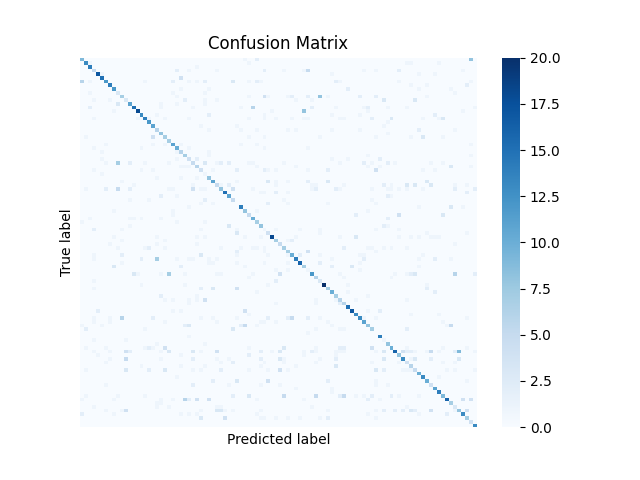
\includegraphics[scale=0.58]{custom_cnn_conf_matrix.png}
	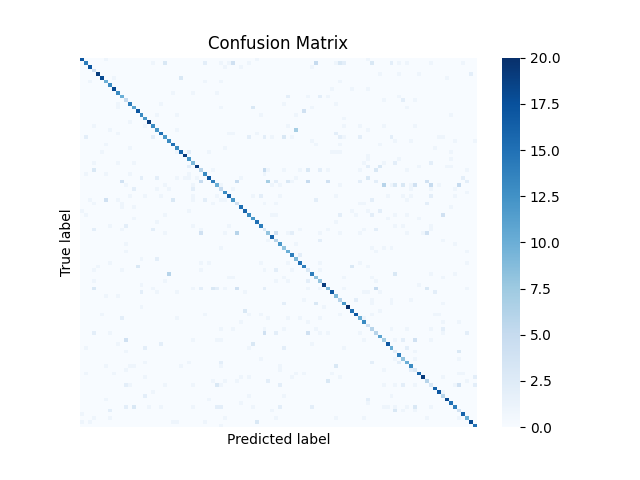
\includegraphics[scale=0.58]{effinet_conf_matrix.png}
	\caption{Custom CNN and Custom EffiNet Confusion Matrices}
\end{figure}

The table below contains the F1 scores on the validation set for all four variants of the models:
\begin{table}[h]
	\centering
	\caption{F1 scores on the validation set of the models used}
	\label{table1}
	\begin{tabular}{cccc}
		\bottomrule
		\multicolumn{2}{|c|}{\textbf{Custom CNN}} &
		\multicolumn{2}{c|}{\textbf{Custom EffiNet}} \\
		\toprule
		\textbf{With Normalization}& \textbf{Without Normalization}& \textbf{Without Normalization}& \textbf{Accuracy} \\
		\midrule
		0.4021 & 0.4132 & 0.5830 & 0.5926 \\
 		\bottomrule
	\end{tabular}
\end{table}

\section{Conclusion}
The technical analysis of the Custom CNN and Custom EfficientNet models reveals their proficiency in image classification tasks. Although the result for the best model was not comparable to something state of the art, it is decent, as it surpassed the baseline by quite a bit.

\newpage

\bibliographystyle{IEEEtran}

%\bibliography{template} %-->reference list is on the template.bib file
\begin{thebibliography}{1.7} 
	\bibitem[1]{effinet}{EfficientNet: Rethinking Model Scaling for Convolutional Neural Networks, Mingxing Tan and Quoc V. Le, 2020} 
\end{thebibliography}

\end{document}